\subsection{Simulatore scelto: Alchemist}\label{subsec:alchemist}
  Alchemist~\cite{alchemist-jos2013} è un meta-simulatore estendibile completamente \engEmph{open-source} che esegue su \engEmph{Java~Virtual~Machine}, nato all'interno dell'Università di Bologna.

  \subsubsection{Simulazione}\label{subsec:introAlchemist}
    In generale, una \emph{simulazione}~\cite{des3} è una riproduzione del modo di operare di un sistema o un processo del mondo reale nel tempo.
    L'imitazione del processo del mondo reale è detta \emph{modello};
    esso risulta essere una riproduzione più o meno semplificata del mondo reale, che viene aggiornata ad ogni passo di esecuzione della simulazione.

    Alchemist rientra nell'archetipo dei simulatori ad eventi discreti (DES)~\cite{des, des2}:
    gli eventi sono strettamente ordinati e vengono eseguiti uno alla volta, determinando il passare del tempo.
    L'idea dietro al progetto è quello di riuscire ad avere un framework di simulazione il più possibile generico, in grado di simulare sistemi di tipologia e complessità diverse, mantenendo le prestazioni dei simulatori non generici (come ad esempio quelli impiegati in ambito chimico~\cite{gillespie1976}).

    Per perseguire questo obiettivo, la progettazione dell'algoritmo è partita dallo studio del lavoro di Gillespie del 1977~\cite{gillespie1977} e di altri scienziati nell'ambito della simulazione chimica.
    Nonostante siano presenti algoritmi in grado di eseguire un numero di reazioni addirittura in tempo costante, la scelta dell'algoritmo è infine ricaduta su una versione migliorata dell'algoritmo SSA di Gillespie, il Next Reaction Method~\cite{nextReactionMethod} di Gibson e Bruck:
    ad ogni passo di simulazione, esso è in grado di selezionare la reazione successiva in tempo costante e richiede un tempo logaritmico per aggiornare le strutture dati interne al termine dell'esecuzione dell'evento.

  \subsubsection{Astrazioni e modello}\label{subsec:modello}
    \begin{figure}[htbp]
      \centering
      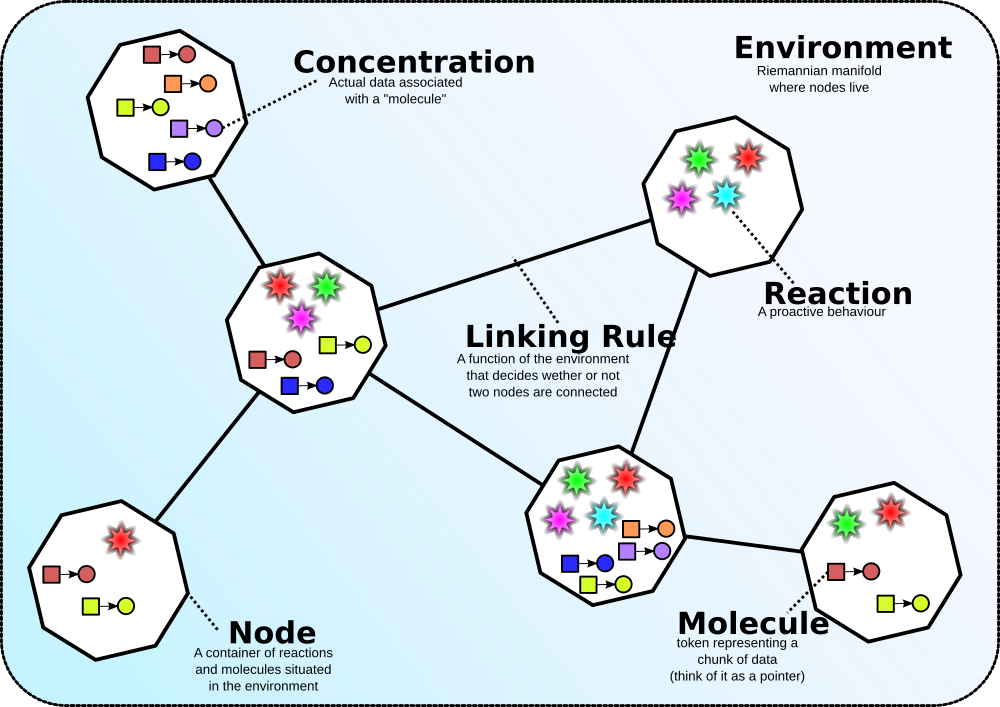
\includegraphics[width=.85\textwidth]{res/fig/alchemist_model.png}
      % \caption[%
      %   Rappresentazione grafica delle diverse entità di Alchemist.

      %   All'interno di un ambiente, che modella il sistema, si trovano i nodi connessi tra loro attraverso dei collegamenti;
      %   ogni nodo è composto da reazioni e molecole, ognuna delle quali ha associata una concentrazione.
      % ]{%
      %   Rappresentazione grafica delle diverse entità di Alchemist.

      %   All'interno di un ambiente, che modella il sistema, si trovano i nodi connessi tra loro attraverso dei collegamenti;
      %   ogni nodo è composto da reazioni e molecole, ognuna delle quali ha associata una concentrazione.

      %   Figura ripresa dal sito ufficiale\footnote{\url{http://alchemistsimulator.github.io}}.
      % }%
      \caption[%
        Rappresentazione grafica delle diverse entità di Alchemist.
      ]{%
        Rappresentazione grafica delle diverse entità di Alchemist.

        Figura ripresa dal sito ufficiale\footnotemark.
      }%
      \label{fig:alchemist:model}
    \end{figure}
    \footnotetext{\url{http://alchemistsimulator.github.io}}

    Il modello di astrazione di Alchemist è ispirato dal lavoro della comunità scientifica nell'ambito dei simulatori a scopo di ricerca chimica e ne riprende dunque la nomenclatura.
    Le entità (visibili in \Cref{fig:alchemist:model}) su cui lavora sono le seguenti:

    \begin{description}
      \item[Molecola]\label{itm:mol}
        Una \emph{Molecola} rappresenta il nome dato ad un particolare dato all'interno di un \emph{Nodo}, del quale ne astrae parte dello stato.

        Un parallelismo con la programmazione imperativa vedrebbe la \emph{Molecola} come un'astrazione del nome di una variabile.

      \item[Concentrazione]\label{itm:conc}
        La \emph{Concentrazione} di una \emph{Molecola} è il valore associato alla proprietà rappresentata dalla \emph{Molecola}.

        Mantenendo il parallelismo con la programmazione imperativa, la \emph{Concentrazione} rappresenterebbe il valore della variabile.

      \item[Nodo]\label{itm:node}
        Il \emph{Nodo} è un contenitore di \emph{Molecole} e \emph{Reazioni} che risiede all'interno di un \emph{Ambiente} e che astrae una singola entità.

      \item[Ambiente]\label{itm:env}
        L'\emph{Ambiente} è l'astrazione che rappresenta lo spazio nella simulazione ed è l'entità che contiene i \emph{Nodi}.

        Esso è in grado di fornire informazioni in merito alla posizione dei \emph{Nodi} nello spazio, alla distanza tra loro e al loro vicinato;
        opzionalmente, l'\emph{Ambiente} può offrire il supporto allo spostamento dei \emph{Nodi}.

      \item[Regola di collegamento]\label{itm:linkr}
        La \emph{Regola di collegamento} è una funzione dello stato corrente dell'\emph{Ambiente} che associa ad ogni \emph{Nodo} un \emph{Vicinato}.

      \item[Vicinato]\label{itm:neigh}
        Un \emph{Vicinato} è un'entità costituita da un \emph{Nodo} detto ``centro'' e da un insieme di altri \emph{Nodi} (i ``vicini'').

        L'astrazione dovrebbe avere un'accezione il più possibile generale e flessibile, in modo da poter modellare qualsiasi tipo di legame di vicinato, non solo spaziale.

        \begin{figure}[htbp]
          \centering
          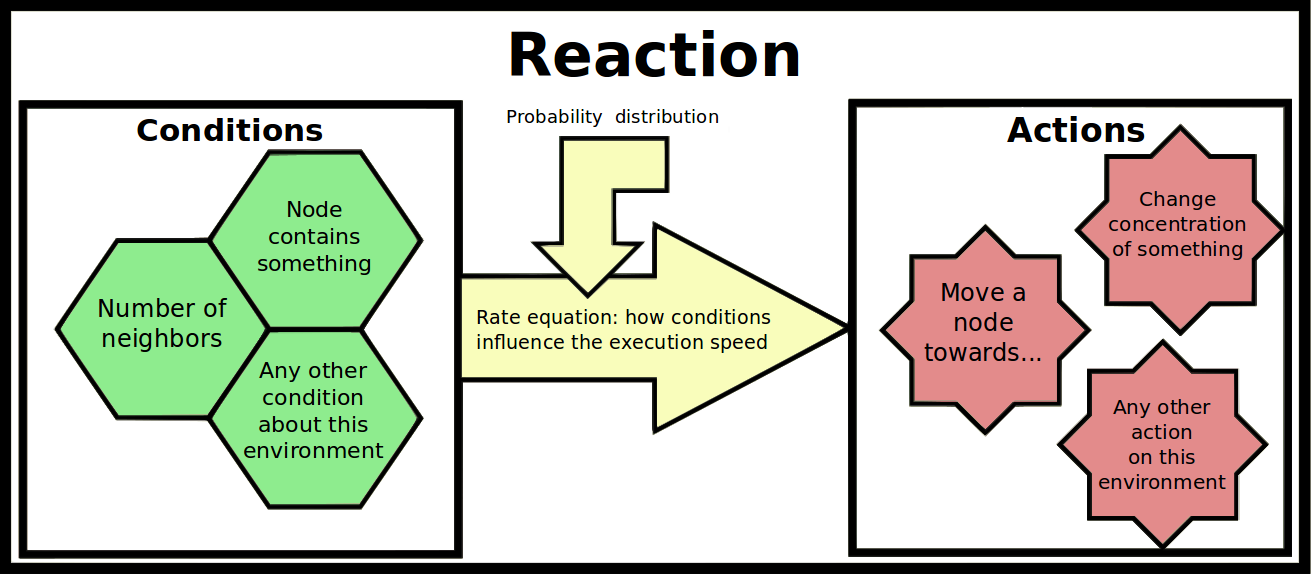
\includegraphics[width=.85\textwidth]{res/fig/alchemist_reaction.png}
          \caption[Rappresentazione grafica della \emph{Reazione}.]{%
              Rappresentazione grafica della \emph{Reazione}.

              % Figura rivisitata da quella disponibile sul sito ufficiale.
          }%
          \label{fig:alchemist:reaction}
        \end{figure}

      \item[Reazione]\label{itm:react}
        Il concetto di \emph{Reazione} è da considerarsi molto più elaborato di quello utilizzato in chimica:
        in questo caso, si può considerare come un insieme di \emph{Condizioni} sullo stato del sistema, che qualora dovessero risultare vere innescherebbero l'esecuzione di un insieme di \emph{Azioni}.

        Una \emph{Reazione} (di cui è si ha una rappresentazione grafica in \Cref{fig:alchemist:reaction}) è dunque un qualsiasi evento che può cambiare lo stato dell'\emph{Ambiente} e si compone di un insieme di \emph{Condizioni}, una o più \emph{Azioni} e una distribuzione temporale.

        La frequenza di accadimento può dipendere da:
        \begin{itemize}
            \item Un tasso statico;
            \item Il valore di ciascuna \emph{Condizione};
            \item Una equazione che combina il tasso statico e il valore delle \emph{Condizioni}, restituendo un ``tasso istantaneo'';
            \item Una distribuzione temporale.
        \end{itemize}

        Ogni \emph{Nodo} è costituito da un insieme (anche vuoto) di \emph{Reazioni}.

      \item[Condizione]\label{itm:cond}
        Una \emph{Condizione} è una funzione che associa un valore numerico e un valore booleano allo stato corrente di un \emph{Ambiente}.

      \item[Azione]\label{itm:act}
        Un'\emph{Azione} è una procedura che provoca una modifica allo stato dell'\emph{Ambiente}.

      \end{description}

  % TODO: inserisci qualcosa su come Alchemist permette a Protelis di girare

  \improvement[inline]{Qui dovrei descrivere anche l'incarnazione di Protelis per Alchemist?}
